\maketitle
\begin{abstract}
\Lang{A boundary in an energy--time diagram requires a declared physical evolution, calibrated responses and a resource with specified units. WR-VII supplies such an interface for finite-dimensional closed unitary dynamics, with energy resource defined as Hamiltonian spectral diameter. A self-contained projector-response argument gives an action certificate and a sharp lower frontier for an observed transition probability. A constant-qubit benchmark then computes the entire compatible generator class, including separated revival windows. At the resource frontier, transition probability selects the spectral diameter but leaves a circle of distinct Hamiltonians. Additional phase-calibrated responses identify this circle for a nonorthogonal final state; at complete transfer, even final-state tomography cannot identify the generator, while an intermediate-time protocol can. Response intervals and independent finite repetitions give separate deterministic and confidence-qualified feasibility certificates. The arguments use established quantum speed-limit, Hamiltonian-identification and concentration tools, with no theorem-priority claim. They certify a boundary of the declared response-and-control model, not an upper energy of reality, a universal lifetime or a cosmological realizability wall.}
{Граница на энергетико-временной диаграмме требует заданной физической эволюции, калиброванных откликов и ресурса с указанными единицами. WR-VII строит такую схему для конечномерной замкнутой унитарной динамики; энергетический ресурс определяется спектральным диаметром гамильтониана. Самостоятельный аргумент для отклика проектора даёт сертификат действия и точный нижний рубеж для наблюдаемой вероятности перехода. Пример с постоянным гамильтонианом кубита затем вычисляет весь совместимый класс генераторов, включая разделённые окна возвратов. На ресурсном рубеже вероятность перехода отбирает спектральный диаметр, но оставляет окружность различных гамильтонианов. Дополнительные фазово-калиброванные отклики идентифицируют эту окружность для неортогонального конечного состояния; при полном переносе даже томография конечного состояния не определяет генератор, тогда как протокол промежуточного времени может его определить. Интервалы отклика и независимые конечные повторения дают отдельные детерминированные сертификаты и сертификаты с гарантией покрытия. Используются известные инструменты квантовых пределов скорости, идентификации гамильтонианов и концентрации; приоритет теорем не заявлен. Удостоверяется граница заданной модели отклика и управления, а не верхняя энергия реальности, универсальное время жизни или космологическая стена реализуемости.}
\end{abstract}
\noindent\textbf{\Lang{Keywords}{Ключевые слова}:} \Lang{energy--time frontier; spectral diameter; quantum response; generator completion; finite confidence; protocol refinement.}{энергетико-временной рубеж; спектральный диаметр; квантовый отклик; достраивание генератора; конечное покрытие; уточнение протокола.}
\smallskip
\begingroup\small\raggedright
\noindent\Lang{Parallel EN/RU texts share all result and equation numbers. REVIEWABLE\_DRAFT; not externally peer reviewed; no WR-VII DOI. Content CC BY 4.0; code MIT.}{Тексты EN/RU имеют общие номера результатов и формул. REVIEWABLE\_DRAFT; внешнего рецензирования нет; DOI WR-VII не присвоен. Текст CC BY 4.0; код MIT.}\par\endgroup
\newpage\tableofcontents\newpage

\section{\Lang{The new obligation: operational frontiers}{Новая задача: операционные рубежи}}\label{sec:scope}
\Lang{WR-I defines response equivalence and identifiable quantities \cite{WRI}; WR-II separates finite consistency from full global realization \cite{WRII}; WR-III studies nonempty response fibres \cite{WRIII}; WR-IV distinguishes complete realizations from history projections \cite{WRIV}. WR-V adds experimental transition descriptions \cite{WRV}, and WR-VI records measured data, structural assumptions and separately justified hard bounds \cite{WRVI}. The WR-VI activity cap is dimensionless. Its numerical threshold cannot acquire units of energy or duration by renaming a parameter.}
{WR-I определяет эквивалентность по откликам и идентифицируемые величины \cite{WRI}; WR-II отделяет конечную согласованность от полной глобальной реализации \cite{WRII}; WR-III изучает непустые слои откликов \cite{WRIII}; WR-IV различает полные реализации и исторические проекции \cite{WRIV}. WR-V добавляет описания экспериментальных переходов \cite{WRV}, а WR-VI фиксирует измеренные данные, структурные предположения и отдельно обоснованные жёсткие границы \cite{WRVI}. Граница активности WR-VI безразмерна. Её численный порог не получает единиц энергии или длительности при переименовании параметра.}

\Lang{The new obligation is to construct a duration-bearing quantum response model and a resource-feasibility region, then ask which generator parameters that region identifies. Classical transition kernels and coherent unitary generators remain distinct carriers. The inherited interface is compatibility with calibrated responses and declared restrictions. Quantum speed limits and Hamiltonian identification already have extensive prior art \cite{AA,ZS}; the contribution here is an explicit, auditable WREH completion calculation, with elementary proofs and stated limitations.}
{Новая задача --- построить квантовую модель отклика с длительностью и областью допустимости ресурсов, а затем выяснить, какие параметры генератора она идентифицирует. Классические ядра переходов и когерентные унитарные генераторы остаются различными носителями. Наследуется схема совместимости с калиброванными откликами и заданными ограничениями. Квантовые пределы скорости и идентификация гамильтонианов имеют обширную предшествующую теорию \cite{AA,ZS}; вклад здесь --- явное проверяемое вычисление достраивания WREH с элементарными доказательствами и указанными ограничениями.}

\Lang{A lower resource frontier asks when one specified response can be produced within a calibrated model. A global realizability boundary would require an independently declared class of complete worlds and a justified response map. These questions have different domains. No upper energy of the Universe or maximum lifetime follows from the construction below.}
{Нижний ресурсный рубеж отвечает, когда один заданный отклик может быть произведён в калиброванной модели. Граница глобальной реализуемости потребовала бы независимо заданного класса полных миров и обоснованного отображения откликов. Это вопросы разных областей. Верхняя энергия Вселенной или максимальное время жизни из следующей конструкции не следуют.}

\section{\Lang{Carrier, clock and energy record}{Носитель, часы и паспорт энергии}}\label{sec:record}
\Lang{Let $\mathcal H=\mathbb C^n$, $n\geq2$. On the calibrated interval $[0,\tau]$, $\tau>0$, a Hermitian Hamiltonian $H(t)$ with integrable operator norm generates the normalized absolutely continuous solution}
{Пусть $\mathcal H=\mathbb C^n$, $n\geq2$. На калиброванном интервале $[0,\tau]$, $\tau>0$, эрмитов гамильтониан $H(t)$ с интегрируемой операторной нормой задаёт нормированное абсолютно непрерывное решение}
\begin{equation}\label{eq:schrodinger}
 i\hbar\dot\psi(t)=H(t)\psi(t),\qquad \|\psi(0)\|=1.
\end{equation}
\Lang{For a fixed orthogonal projector $Q$, prepare $Q\psi(0)=0$ and measure its final Born probability. Define}
{Для фиксированного ортогонального проектора $Q$ подготовим $Q\psi(0)=0$ и измерим его конечную вероятность Борна. Определим}
\begin{equation}\label{eq:resource}
 p(t)=\langle\psi(t),Q\psi(t)\rangle,\qquad
 D(t)=\lambda_{\max}(H(t))-\lambda_{\min}(H(t)),\qquad
 A=\frac{1}{2\hbar}\int_0^\tau D(t)\,dt.
\end{equation}
\Lang{$D$ and its pointwise upper cap $E\geq0$ have units of joules; $\tau$ has units of seconds; $A$ is dimensionless. Spectral diameter is invariant under $H(t)\mapsto H(t)+c(t)I$. Such a shift changes only a global state phase. The resource is neither consumed work nor mean energy, and is not the state's energy standard deviation. A claim involving those quantities needs a different record. The finite-dimensional closed-system law, clock, preparation, measurement and hard diameter cap are supplied assumptions that must be calibrated in an apparatus.}
{$D$ и его поточечная верхняя граница $E\geq0$ измеряются в джоулях; $\tau$ --- в секундах; $A$ безразмерно. Спектральный диаметр инвариантен при $H(t)\mapsto H(t)+c(t)I$. Такой сдвиг меняет лишь глобальную фазу состояния. Ресурс не является затраченной работой или средней энергией и не равен стандартному отклонению энергии состояния. Для утверждений об этих величинах нужен другой паспорт. Конечномерный закон замкнутой системы, часы, подготовка, измерение и жёсткая граница диаметра являются заданными предположениями, которые требуется калибровать в установке.}

\begin{definition}[\Lang{Operational completion class}{Операционный класс достраиваний}]\label{def:completion}
\Lang{With the preceding carrier and protocol fixed, $\mathcal C(E,\tau,J)$ consists of Hamiltonian histories satisfying $D(t)\leq E$ almost everywhere and $p(\tau)\in J$, where $J\subseteq[0,1]$ is the supplied response set. A constant-qubit subclass will be stated separately.}
{При фиксированных предыдущих носителе и протоколе $\mathcal C(E,\tau,J)$ состоит из историй гамильтониана, удовлетворяющих $D(t)\leq E$ почти всюду и $p(\tau)\in J$, где $J\subseteq[0,1]$ --- заданное множество откликов. Подкласс постоянных гамильтонианов кубита будет указан отдельно.}
\end{definition}
\Lang{Nonemptiness says that at least one allowed generator produces the response. It does not require every allowed generator to do so, or identify the actual generator. The evolution duration excludes preparation, readout and resetting overhead. An inference about total experimental time must additionally account for repetitions and those durations.}
{Непустота означает, что хотя бы один допустимый генератор производит отклик. Она не требует этого от каждого допустимого генератора и не идентифицирует фактический генератор. Длительность эволюции исключает время подготовки, считывания и сброса. Вывод о полном времени эксперимента должен дополнительно учитывать повторения и эти длительности.}

\section{\Lang{A sharp response-action certificate}{Точный сертификат действия для отклика}}\label{sec:action}
\begin{theorem}[\Lang{Projector-response action bound}{Граница действия для отклика проектора}]\label{thm:action}
\Lang{Under~\eqref{eq:schrodinger}--\eqref{eq:resource},}
{При~\eqref{eq:schrodinger}--\eqref{eq:resource}}
\begin{equation}\label{eq:actionbound}
 \arcsin\sqrt{p(\tau)}\leq A.
\end{equation}
\end{theorem}
\begin{proof}
\Lang{Set $u=Q\psi$ and $v=(I-Q)\psi$. Their norms are $\sqrt p$ and $\sqrt{1-p}$, and $u\perp v$. For $c=(\lambda_{\max}H+\lambda_{\min}H)/2$, $\|H-cI\|=D/2$. The commutator formula therefore gives, almost everywhere,}
{Положим $u=Q\psi$ и $v=(I-Q)\psi$. Их нормы равны $\sqrt p$ и $\sqrt{1-p}$, и $u\perp v$. Для $c=(\lambda_{\max}H+\lambda_{\min}H)/2$ выполнено $\|H-cI\|=D/2$. Поэтому формула коммутатора почти всюду даёт}
\begin{equation}\label{eq:derivative}
 |\dot p|\leq\frac{2}{\hbar}|\langle u,(H-cI)v\rangle|
 \leq\frac{D}{\hbar}\sqrt{p(1-p)}.
\end{equation}
\[ F_\eta(x)=\int_0^x\frac{ds}{2\sqrt{(s+\eta)(1-s+\eta)}},\qquad\eta>0. \]
\Lang{To handle $p=0,1$ without dividing by zero, for $\eta>0$ use the regularized antiderivative displayed above. Its derivative is bounded on $[0,1]$ and the absolutely continuous chain rule gives $|dF_\eta(p)/dt|\leq D/(2\hbar)$. Integrate from $p(0)=0$, then let $\eta\downarrow0$. Monotone convergence of this nonnegative integrand gives $F_\eta(x)\to\arcsin\sqrt x$, including both endpoints.}
{Чтобы обработать $p=0,1$ без деления на ноль, для $\eta>0$ используем регуляризованную первообразную, записанную выше. Его производная ограничена на $[0,1]$, и правило цепочки для абсолютно непрерывных функций даёт $|dF_\eta(p)/dt|\leq D/(2\hbar)$. Проинтегрируем от $p(0)=0$, затем устремим $\eta\downarrow0$. Монотонная сходимость неотрицательного подынтегрального выражения даёт $F_\eta(x)\to\arcsin\sqrt x$, включая оба конца.}
\end{proof}

\begin{corollary}[\Lang{Sharp energy--duration frontier}{Точный энергетико-временной рубеж}]\label{cor:frontier}
\Lang{If $D(t)\leq E$, an exact response $p\in[0,1]$ requires $E\tau\geq2\hbar\arcsin\sqrt p$. Conversely, on a qubit with $\psi(0)=|0\rangle$ and $Q=|1\rangle\langle1|$, this condition is sufficient. Its full reachable probability set is}
{Если $D(t)\leq E$, точный отклик $p\in[0,1]$ требует $E\tau\geq2\hbar\arcsin\sqrt p$. Обратно, для кубита с $\psi(0)=|0\rangle$ и $Q=|1\rangle\langle1|$ это условие достаточно. Полное множество достижимых вероятностей равно}
\begin{equation}\label{eq:reachable}
 \mathcal R(E,\tau)=[0,\sin^2(\min\{C,\pi/2\})],\qquad C=\frac{E\tau}{2\hbar}.
\end{equation}
\end{corollary}
\begin{proof}
\Lang{Necessity follows from $A\leq C$. For sufficiency set $\theta=\arcsin\sqrt p$ and $H=(\hbar\theta/\tau)\sigma_x$. Its diameter is $2\hbar\theta/\tau\leq E$ and its final transition probability is $\sin^2\theta=p$. For $p=0$ use $H=0$. Every probability in~\eqref{eq:reachable} has this construction; none above it satisfies the action bound.}
{Необходимость следует из $A\leq C$. Для достаточности положим $\theta=\arcsin\sqrt p$ и $H=(\hbar\theta/\tau)\sigma_x$. Его диаметр равен $2\hbar\theta/\tau\leq E$, а конечная вероятность перехода --- $\sin^2\theta=p$. Для $p=0$ используем $H=0$. Каждая вероятность из~\eqref{eq:reachable} имеет такую конструкцию; ни одна более высокая вероятность не удовлетворяет границе действия.}
\end{proof}
\Lang{This is a quantum speed certificate in a supplied unitary model, related to the established geometric energy--time setting \cite{AA}. At complete transfer it gives $E\tau\geq\pi\hbar$. It is not a general energy--time product law for arbitrary physical objects. Sharpness uses a freely chosen transverse qubit generator; a hardware control alphabet or inaccessible axes can make the actual attainable set smaller.}
{Это квантовый сертификат скорости в заданной унитарной модели, связанный с известной геометрической энергетико-временной постановкой \cite{AA}. При полном переносе он даёт $E\tau\geq\pi\hbar$. Это не общий закон произведения энергии и времени для произвольных физических объектов. Точность достигается свободным выбором поперечного генератора кубита; аппаратный набор управлений или недоступные оси могут уменьшить фактически достижимое множество.}

\Lang{For a time-independent $H$ and orthogonalization, the Mandelstam--Tamm and Margolus--Levitin bounds use, respectively, the state's energy spread $\Delta H$ and mean energy above ground $\bar\varepsilon=\langle H\rangle-\lambda_{\min}(H)$ \cite{ML,GLM}. For positive denominators they read}
{Для постоянного $H$ при ортогонализации граница Мандельштама--Тамма использует разброс энергии состояния $\Delta H$, а граница Марголуса--Левитина --- среднюю энергию над основным уровнем $\bar\varepsilon=\langle H\rangle-\lambda_{\min}(H)$ \cite{ML,GLM}. Для положительных знаменателей получаем}
\[
 \tau_\perp\geq\frac{\pi\hbar}{2\Delta H},\qquad
 \tau_\perp\geq\frac{\pi\hbar}{2\bar\varepsilon}.
\]
\Lang{Since $\Delta H\leq D/2$, a state-specific spread can give a stronger bound than the diameter-only orthogonalization certificate. The mean-energy bound is stronger than $\pi\hbar/D$ when $\bar\varepsilon<D/2$; it does not uniformly improve it. For the transverse frontier family at complete transfer, $\Delta H=\bar\varepsilon=E/2$ and the three bounds agree. These state resources are not supplied inputs to Theorem~\ref{thm:action}, and the static mean-energy formula is not applied to arbitrary $H(t)$. Corollary~\ref{cor:frontier} is sharp over its freely controlled diameter-constrained class, not an optimal time estimate for every fixed state and Hamiltonian.}
{Поскольку $\Delta H\leq D/2$, заданный разброс энергии состояния может дать более сильную границу, чем сертификат ортогонализации только по диаметру. Граница средней энергии сильнее $\pi\hbar/D$ при $\bar\varepsilon<D/2$; равномерного усиления она не даёт. Для поперечного порогового семейства при полном переносе выполнено $\Delta H=\bar\varepsilon=E/2$, и три границы совпадают. Эти ресурсы состояния не являются заданными входами теоремы~\ref{thm:action}, а статическая формула средней энергии не применяется к произвольному $H(t)$. Следствие~\ref{cor:frontier} точно по свободно управляемому классу с ограниченным диаметром, но не является оптимальной оценкой времени для каждого фиксированного состояния и гамильтониана.}

\section{\Lang{Complete constant-qubit generator fibre}{Полный слой постоянных генераторов кубита}}\label{sec:fibre}
\Lang{Fix the computational basis and calibrated laboratory axes. Remove the scalar identity term, and write every nonzero constant traceless Hermitian qubit generator as}
{Зафиксируем вычислительный базис и калиброванные лабораторные оси. Удалим скалярный член единичной матрицы и запишем каждый ненулевой постоянный бесследовый эрмитов генератор кубита как}
\begin{equation}\label{eq:qubit}
 \begin{gathered}
 H=\frac d2\,\mathbf n\cdot\boldsymbol\sigma,\quad
 0<d\leq E,\quad\|\mathbf n\|=1,\quad\phi=\frac{d\tau}{2\hbar},\\
 U(\tau)=\cos\phi\,I-i\sin\phi\,\mathbf n\cdot\boldsymbol\sigma.
 \end{gathered}
\end{equation}
\Lang{Here $d$ is spectral diameter, not Hilbert-space dimension. In this section the Hilbert space is fixed as $\mathbb C^2$. For preparation $|0\rangle$ and the $|1\rangle$ projector, direct multiplication gives}
{Здесь $d$ --- спектральный диаметр, а не размерность гильбертова пространства. В этом разделе пространство фиксировано как $\mathbb C^2$. Для подготовки $|0\rangle$ и проектора $|1\rangle$ прямое умножение даёт}
\begin{equation}\label{eq:qubitresponse}
 p=(1-n_z^2)\sin^2\phi.
\end{equation}

\begin{theorem}[\Lang{All compatible constant generators}{Все совместимые постоянные генераторы}]\label{thm:fibre}
\Lang{For $0<p<1$, let $\theta=\arcsin\sqrt p$. The constant-generator completion class is parameterized by}
{Для $0<p<1$ пусть $\theta=\arcsin\sqrt p$. Класс достраиваний постоянных генераторов параметризуется как}
\begin{equation}\label{eq:windows}
 \begin{gathered}
 \phi\in\left(\bigcup_{m\geq0}[m\pi+\theta,(m+1)\pi-\theta]\right)\cap[0,C],\\
 n_z=\pm\sqrt{1-\frac p{\sin^2\phi}},\qquad
 (n_x,n_y)=\frac{\sqrt p}{|\sin\phi|}(\cos\beta,\sin\beta).
 \end{gathered}
\end{equation}
\Lang{with $\beta\in\mathbb R/(2\pi\mathbb Z)$ and $d=2\hbar\phi/\tau$. At window endpoints the two signs coincide. The number of nonempty separated phase windows is zero for $C<\theta$, and otherwise $1+\lfloor(C-\theta)/\pi\rfloor$.}
{где $\beta\in\mathbb R/(2\pi\mathbb Z)$ и $d=2\hbar\phi/\tau$. На концах окон два знака совпадают. Число непустых разделённых окон фаз равно нулю при $C<\theta$, а иначе $1+\lfloor(C-\theta)/\pi\rfloor$.}
\end{theorem}
\begin{proof}
\Lang{Equation~\eqref{eq:qubitresponse} requires $\sin^2\phi\geq p$ and fixes $n_z^2$. On each nonnegative half-period, this inequality is exactly the displayed interval. The transverse magnitude follows from unit normalization, and its azimuth is unrestricted. Conversely these parameters satisfy~\eqref{eq:qubitresponse} and $d\leq E$. A window is nonempty exactly when $m\pi+\theta\leq C$. Distinct windows are separated by forbidden phase gaps, so the stated count follows.}
{Уравнение~\eqref{eq:qubitresponse} требует $\sin^2\phi\geq p$ и фиксирует $n_z^2$. На каждом неотрицательном полупериоде это неравенство задаёт в точности показанный интервал. Поперечный модуль следует из единичной нормировки, а азимут свободен. Обратно, такие параметры удовлетворяют~\eqref{eq:qubitresponse} и $d\leq E$. Окно непусто ровно при $m\pi+\theta\leq C$. Различные окна разделены запрещёнными промежутками фаз, откуда следует указанное число.}
\end{proof}

\begin{corollary}[\Lang{A frontier can retain generator ambiguity}{Рубеж может сохранять неоднозначность генератора}]\label{cor:circle}
\Lang{For $0<p\leq1$ and $C=\theta$, the constant-qubit class is the circle}
{Для $0<p\leq1$ и $C=\theta$ класс постоянных гамильтонианов кубита является окружностью}
\begin{equation}\label{eq:circle}
 H_\beta=\frac E2(\cos\beta\,\sigma_x+\sin\beta\,\sigma_y),
 \qquad \beta\in\mathbb R/(2\pi\mathbb Z).
\end{equation}
\Lang{Thus the exact frontier identifies $d=E$ in this subclass, but not $H$.}
{Поэтому точный рубеж идентифицирует $d=E$ в этом подклассе, но не $H$.}
\end{corollary}
\begin{proof}
\Lang{At $C=\theta$ the only allowed phase is $\theta$, and~\eqref{eq:qubitresponse} forces $n_z=0$. Each distinct azimuth gives a distinct traceless operator. For $p=1$, $\theta=\pi/2$ and the same argument applies directly.}
{При $C=\theta$ единственная допустимая фаза равна $\theta$, и~\eqref{eq:qubitresponse} вынуждает $n_z=0$. Каждый различный азимут даёт различный бесследовый оператор. Для $p=1$, $\theta=\pi/2$, тот же аргумент применяется напрямую.}
\end{proof}
\Lang{This is a pointwise instance of the WR-I distinction between an identifiable quantity and its full carrier object \cite{WRI}: $H\mapsto D(H)$ is constant on this constrained exact-response fibre, while $H$ itself is not. It does not assert that diameter is identifiable on every response fibre of the entire generator carrier.}
{Это точечный пример различия WR-I между идентифицируемой величиной и полным объектом носителя \cite{WRI}: $H\mapsto D(H)$ постоянно на этом ограниченном слое точного отклика, тогда как сам $H$ неоднозначен. Идентифицируемость диаметра на каждом слое откликов всего носителя генераторов не утверждается.}
\Lang{Here the minimum resource is attained, by a circle of generators. This exact-data degeneracy differs from WR-II v0.5, Example~10.19 \cite{WRII}, and WR-VI v0.2, Corollary~5.3 \cite{WRVI}, where a nonclosed admissible class has an unattained infimum. In WR-VI the additional irreducibility requirement excludes the minimizing matrix. No analogous strict exclusion is imposed on the present constant-qubit frontier family.}
{Здесь минимум ресурса достигается, причём на окружности генераторов. Это вырождение при точных данных отличается от примера~10.19 WR-II v0.5 \cite{WRII} и следствия~5.3 WR-VI v0.2 \cite{WRVI}, где незамкнутый допустимый класс имеет недостигаемый инфимум. В WR-VI дополнительное требование неприводимости исключает минимизирующую матрицу. Аналогичного строгого исключения в настоящем постоянном пороговом семействе кубита нет.}

\Lang{The azimuth is not declared a physical gauge: the laboratory $x,y$ axes are fixed and additional calibrated probes can distinguish it. Only scalar identity shifts were removed. For $p=1$, allowed phases are the points $\pi/2+m\pi$, each with a transverse circle. For $p=0$, phases $m\pi$ allow every axis, while other phases require $n_z=\pm1$. At $d=0$, all axis labels represent the same zero operator. These endpoint cases must not be obtained by dividing~\eqref{eq:windows} by zero.}
{Азимут не объявляется физической калибровочной свободой: лабораторные оси $x,y$ фиксированы, и дополнительные калиброванные зонды могут его различить. Удалены только скалярные сдвиги единичной матрицы. Для $p=1$ допустимые фазы --- точки $\pi/2+m\pi$, каждая с поперечной окружностью. Для $p=0$ фазы $m\pi$ допускают любую ось, а остальные фазы требуют $n_z=\pm1$. При $d=0$ все метки оси представляют один нулевой оператор. Эти граничные случаи нельзя получать делением~\eqref{eq:windows} на ноль.}

\section{\Lang{Which additional protocol identifies the circle?}{Какой дополнительный протокол идентифицирует окружность?}}\label{sec:probes}
\Lang{For the frontier family~\eqref{eq:circle}, calibrated Pauli means in fresh preparations at the same duration are}
{Для порогового семейства~\eqref{eq:circle} калиброванные средние Паули на новых подготовках при той же длительности равны}
\begin{equation}\label{eq:bloch}
 (r_x,r_y,r_z)=(\sin\beta\sin2\theta,\;-\cos\beta\sin2\theta,\;\cos2\theta).
\end{equation}
\begin{theorem}[\Lang{State identification differs from generator identification}{Идентификация состояния отличается от идентификации генератора}]\label{thm:probes}
\Lang{Restrict to the constant frontier family. If $0<p<1$, exact $r_x,r_y$ at $\tau$ identify $\beta$ modulo $2\pi$, hence $H$. If $p=1$, the complete final density operator is the same for every $\beta$, so no final-state observable at that duration identifies $H$. At $p=1$, exact $r_x,r_y$ on separate preparations evolved for $\tau/2$ identify $\beta$.}
{Ограничимся постоянным пороговым семейством. Если $0<p<1$, точные $r_x,r_y$ при $\tau$ идентифицируют $\beta$ по модулю $2\pi$, а значит $H$. Если $p=1$, полная конечная матрица плотности одинакова для каждого $\beta$, поэтому ни одна наблюдаемая конечного состояния при этой длительности не идентифицирует $H$. При $p=1$ точные $r_x,r_y$ на отдельных подготовках с эволюцией в течение $\tau/2$ идентифицируют $\beta$.}
\end{theorem}
\begin{proof}
\Lang{Direct multiplication of $U|0\rangle=(\cos\theta,-i e^{i\beta}\sin\theta)^T$ gives~\eqref{eq:bloch}. For $0<p<1$, $s=\sin2\theta=2\sqrt{p(1-p)}>0$, so $(r_x/s,-r_y/s)=(\sin\beta,\cos\beta)$ determines the azimuth. For $p=1$, $\theta=\pi/2$, and the density operator is $|1\rangle\langle1|$ independently of the azimuth. At half-duration the same constant generator has phase $\pi/4$, giving $(r_x,r_y)=(\sin\beta,-\cos\beta)$.}
{Прямое умножение $U|0\rangle=(\cos\theta,-i e^{i\beta}\sin\theta)^T$ даёт~\eqref{eq:bloch}. Для $0<p<1$ выполнено $s=\sin2\theta=2\sqrt{p(1-p)}>0$, поэтому $(r_x/s,-r_y/s)=(\sin\beta,\cos\beta)$ определяет азимут. Для $p=1$, $\theta=\pi/2$, матрица плотности равна $|1\rangle\langle1|$ независимо от азимута. При половинной длительности тот же постоянный генератор имеет фазу $\pi/4$ и даёт $(r_x,r_y)=(\sin\beta,-\cos\beta)$.}
\end{proof}
\Lang{The half-duration measurement is performed on another preparation, rather than inserted into the original evolution. Exact additional means are new data, not values inferred from the first transition probability. The constant-generator and exact-frontier assumptions are essential; this is not a complete identification theorem for arbitrary time-dependent controls. Division by $2\sqrt{p(1-p)}$ also reveals a finite-resolution difficulty near both response endpoints. A finite tomography design requires its own sampling and calibration analysis.}
{Измерение при половинной длительности выполняется на другой подготовке, а не вставляется в исходную эволюцию. Точные дополнительные средние являются новыми данными, а не величинами, выведенными из первой вероятности перехода. Предположения постоянного генератора и точного рубежа существенны; это не полная теорема идентификации произвольных зависящих от времени управлений. Деление на $2\sqrt{p(1-p)}$ также показывает трудность конечного разрешения вблизи обоих концов отклика. Конечная схема томографии требует собственного анализа выборки и калибровки.}

\section{\Lang{Calibrated numerical benchmark and response intervals}{Калиброванный численный пример и интервалы отклика}}\label{sec:benchmark}
\Lang{Write $\nu=E/h$, where $h=2\pi\hbar$. With a supplied spectral-gap cap $\nu=10\,\mathrm{MHz}$ and target $p=1/4$, $\theta=\pi/6$ and}
{Запишем $\nu=E/h$, где $h=2\pi\hbar$. При заданной границе спектрального разрыва $\nu=10\,\mathrm{MHz}$ и целевом $p=1/4$ выполнено $\theta=\pi/6$ и}
\begin{equation}\label{eq:units}
 \tau_{\min}=\frac{\theta}{\pi\nu}=\frac1{6\nu}
 =\frac{50}{3}\,\mathrm{ns},\qquad E=h\nu=6.62607015\times10^{-27}\,\mathrm J.
\end{equation}
\Lang{The exact SI value $h=6.62607015\times10^{-34}\,\mathrm{J\,s}$ is supplied by the defining-constant convention \cite{BIPM}. The numerical frequency is a chosen calibrated-model input, not a measurement reported from a device. At the frontier, $H_0$ and $H_{\pi/2}$ have the same transition probability but different $(r_x,r_y)$: $(0,-\sqrt3/2)$ and $(\sqrt3/2,0)$. Complete transfer at the same cap takes at least $50\,\mathrm{ns}$, retains the same circle, and is resolved by the proposed probes at $25\,\mathrm{ns}$.}
{Точное значение СИ $h=6.62607015\times10^{-34}\,\mathrm{J\,s}$ задаётся соглашением об определяющей постоянной \cite{BIPM}. Численная частота является выбранным входом калиброванной модели, а не измерением, выполненным на приборе. На рубеже $H_0$ и $H_{\pi/2}$ имеют одинаковую вероятность перехода, но разные $(r_x,r_y)$: $(0,-\sqrt3/2)$ и $(\sqrt3/2,0)$. Полный перенос при той же границе занимает не менее $50\,\mathrm{ns}$, сохраняет ту же окружность и различается предложенными зондами при $25\,\mathrm{ns}$.}

\begin{figure}[htbp]\centering
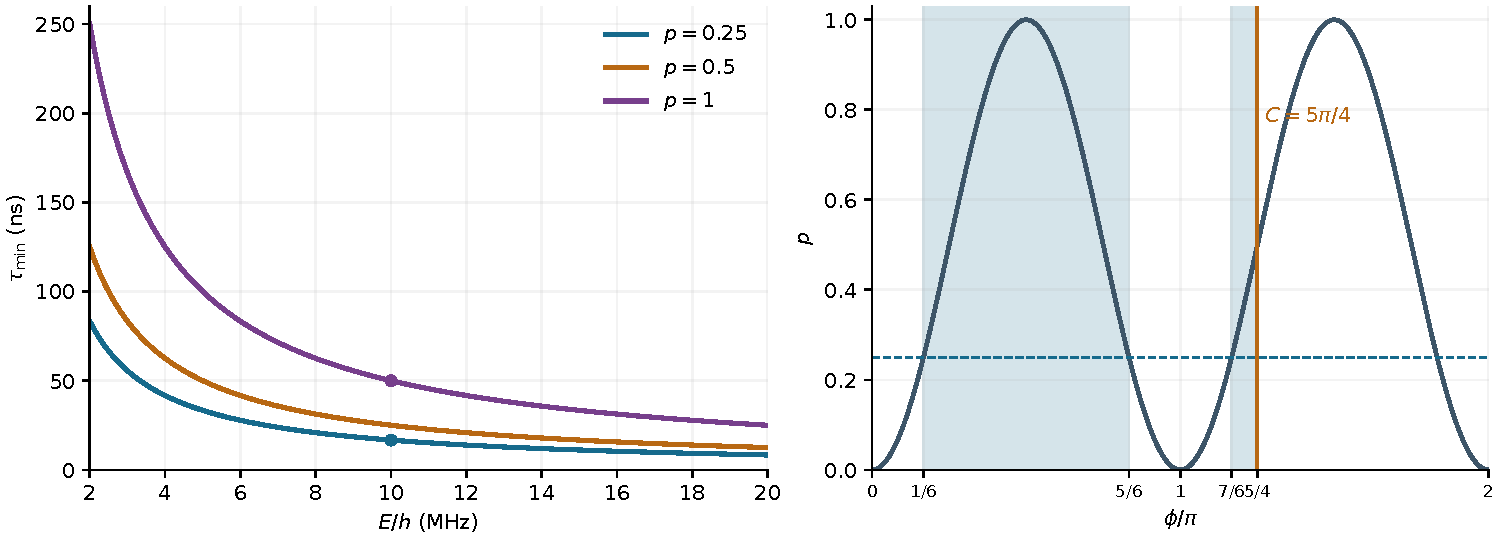
\includegraphics[width=\linewidth]{figures/frontiers.pdf}
\caption{\Lang{Left: conditional resource frontiers for three responses, with spectral diameter expressed as $E/h$ and duration in nanoseconds. Right: allowed phases for $p=1/4$; a larger resource budget can admit a second separated window. These are analytic model curves, not experimental observations.}{Слева: условные ресурсные рубежи для трёх откликов со спектральным диаметром в единицах $E/h$ и длительностью в наносекундах. Справа: допустимые фазы для $p=1/4$; больший ресурсный бюджет может допустить второе разделённое окно. Это аналитические модельные кривые, а не экспериментальные наблюдения.}}\label{fig:frontiers}
\end{figure}

\begin{proposition}[\Lang{Closed response intervals have a lower-endpoint frontier}{Замкнутые интервалы отклика имеют рубеж по нижнему концу}]\label{prop:interval}
\Lang{On the qubit carrier of Corollary~\ref{cor:frontier}, let $J=[p_-,p_+]\subseteq[0,1]$ be nonempty. Then}
{На носителе кубита из следствия~\ref{cor:frontier} пусть $J=[p_-,p_+]\subseteq[0,1]$ непуст. Тогда}
\begin{equation}\label{eq:intervalfrontier}
 \mathcal C(E,\tau,J)\ne\varnothing
 \quad\Longleftrightarrow\quad
 E\tau\geq2\hbar\arcsin\sqrt{p_-}.
\end{equation}
\end{proposition}
\begin{proof}
\Lang{Any compatible $p\in J$ is at least $p_-$, so necessity follows from the monotone action certificate. For sufficiency, the constant transverse construction at $p_-$ belongs to the class. In particular, $p_-=0$ gives the zero generator for every budget.}
{Любое совместимое $p\in J$ не меньше $p_-$, поэтому необходимость следует из монотонного сертификата действия. Для достаточности постоянная поперечная конструкция при $p_-$ принадлежит классу. В частности, $p_-=0$ даёт нулевой генератор при любом бюджете.}
\end{proof}
\Lang{The quantifier is existence of one probability in the observed interval, not one generator that simultaneously produces all probabilities. A deterministic interval has no statistical coverage by definition. A nonzero lower endpoint gives a robust lower certificate within this observation record; if zero is allowed, that certificate disappears.}
{Квантор означает существование одной вероятности из наблюдаемого интервала, а не одного генератора, одновременно производящего все вероятности. Детерминированный интервал по определению не имеет статистической гарантии покрытия. Ненулевой нижний конец даёт устойчивый нижний сертификат в этом паспорте наблюдения; если допускается ноль, сертификат исчезает.}

\section{\Lang{Finite repetitions and qualified exclusion}{Конечные повторения и исключение с гарантией покрытия}}\label{sec:sampling}
\Lang{For a prespecified duration and generator stable across fresh preparations, suppose recorded binary outcomes $X_1,\ldots,X_N$ are independent and identically distributed Bernoulli variables with mean $\mu$. Calibration supplies a uniform bound $|\mu-p(\tau)|\leq\delta$, $\delta\geq0$, including any stated preparation/readout bias. Fix $N$ and $0<\alpha<1$ before inspecting outcomes. Define}
{Для заранее выбранной длительности и генератора, стабильного между новыми подготовками, предположим, что записанные бинарные исходы $X_1,\ldots,X_N$ являются независимыми одинаково распределёнными величинами Бернулли со средним $\mu$. Калибровка задаёт равномерную границу $|\mu-p(\tau)|\leq\delta$, $\delta\geq0$, включая заявленное смещение подготовки и считывания. Зафиксируем $N$ и $0<\alpha<1$ до просмотра исходов. Определим}
\begin{equation}\label{eq:confidence}
 \widehat p=\frac1N\sum_iX_i,\qquad
 r_N=\sqrt{\frac{\log(2/\alpha)}{2N}},\qquad
 J_N=[\max\{0,\widehat p-r_N-\delta\},\min\{1,\widehat p+r_N+\delta\}].
\end{equation}
\begin{proposition}[\Lang{Confidence-qualified resource certificate}{Ресурсный сертификат с гарантией покрытия}]\label{prop:confidence}
\Lang{With probability at least $1-\alpha$, $p(\tau)\in J_N$. On that event every compatible closed unitary model obeys $E\tau\geq2\hbar\arcsin\sqrt{\max\{0,\widehat p-r_N-\delta\}}$. Declaring the stated model infeasible only when its cap violates this inequality has false-exclusion probability at most $\alpha$, under the supplied sampling and calibration assumptions.}
{С вероятностью не менее $1-\alpha$ выполнено $p(\tau)\in J_N$. На этом событии каждая совместимая замкнутая унитарная модель удовлетворяет $E\tau\geq2\hbar\arcsin\sqrt{\max\{0,\widehat p-r_N-\delta\}}$. Объявление заданной модели несовместимой только при нарушении её границей этого неравенства имеет вероятность ложного исключения не больше $\alpha$ при заданных предположениях выборки и калибровки.}
\end{proposition}
\begin{proof}
\Lang{For one Bernoulli variable set $g(s)=\log\mathbb E e^{s(X-\mu)}$. Then $g(0)=g'(0)=0$ and $g''(s)$ is the variance of a tilted Bernoulli law, at most $1/4$, hence $g(s)\leq s^2/8$. Independence and the exponential Markov inequality give each tail at deviation $r$ a bound $e^{-2Nr^2}$ after optimizing $s=4r$ (and using the negative sign for the lower tail). The two-tail bound is $2e^{-2Nr^2}$, the Bernoulli case of Hoeffding's inequality \cite{Hoeffding}. At $r=r_N$ it is $\alpha$. The bias bound enlarges the interval by $\delta$, and Theorem~\ref{thm:action} gives the resource conclusion. Under a true capped model, exclusion can occur only outside the coverage event.}
{Для одной величины Бернулли положим $g(s)=\log\mathbb E e^{s(X-\mu)}$. Тогда $g(0)=g'(0)=0$, а $g''(s)$ является дисперсией наклонённого закона Бернулли и не превышает $1/4$, откуда $g(s)\leq s^2/8$. Независимость и экспоненциальное неравенство Маркова дают для каждого хвоста при отклонении $r$ границу $e^{-2Nr^2}$ после оптимизации $s=4r$ (с отрицательным знаком для нижнего хвоста). Двухсторонняя граница равна $2e^{-2Nr^2}$ --- случай Бернулли неравенства Хёффдинга \cite{Hoeffding}. При $r=r_N$ она равна $\alpha$. Граница смещения расширяет интервал на $\delta$, а теорема~\ref{thm:action} даёт ресурсный вывод. При истинной модели с такой границей исключение возможно только вне события покрытия.}
\end{proof}
\Lang{This is a conservative coverage construction, not a necessary sample-size law or an optimal discrimination protocol. Adaptive stopping and drift require additional analysis. Increasing $N$ reduces the sampling term but not the supplied bias floor. For $N=512$, 128 recorded successes, $\alpha=0.05$ and $\delta=0.01$, the lower endpoint is approximately $0.17998$; with $E/h=10\,\mathrm{MHz}$ its time certificate is approximately $13.95\,\mathrm{ns}$. These are synthetic benchmark counts. At least $N\tau$ of evolution time is spent in sequential repetitions, with overhead added separately; parallel hardware changes that accounting.}
{Это консервативная конструкция покрытия, а не необходимый закон объёма выборки или оптимальный протокол различения. Адаптивная остановка и дрейф требуют дополнительного анализа. Увеличение $N$ уменьшает выборочный член, но не заданный предел смещения. Для $N=512$, 128 записанных успехов, $\alpha=0.05$ и $\delta=0.01$ нижний конец приблизительно равен $0.17998$; при $E/h=10\,\mathrm{MHz}$ временной сертификат составляет приблизительно $13.95\,\mathrm{ns}$. Это синтетические числа для примера. При последовательных повторениях расходуется не менее $N\tau$ времени эволюции; накладные длительности добавляются отдельно, а параллельная аппаратура меняет этот учёт.}

\section{\Lang{Physical boundaries and global realizability}{Физические границы и глобальная реализуемость}}\label{sec:ceilings}
\Lang{The attainable-response boundary and an internal structural wall are distinct WR-III objects \cite{WRIII}. For fixed $E,\tau$ with $0<C<\pi/2$, declare the response manifold $M=(0,1)$. Equation~\eqref{eq:reachable} gives the full-dimensional image $\mathcal R(E,\tau)\cap M=(0,\sin^2 C]$, whose boundary in $M$ is its upper endpoint. For a target $p\in M$, this upper-boundary condition rewrites as the energy--duration frontier in Corollary~\ref{cor:frontier}. This is a response-boundary identification with a specified ambient space. It is not an assertion of failure of local fibre triviality; such a structural-wall theorem would need a separately declared total carrier, topology and response map.}
{Граница достижимых откликов и внутренняя структурная стена являются различными объектами WR-III \cite{WRIII}. При фиксированных $E,\tau$ с $0<C<\pi/2$ зададим многообразие откликов $M=(0,1)$. Уравнение~\eqref{eq:reachable} даёт полноразмерный образ $\mathcal R(E,\tau)\cap M=(0,\sin^2 C]$, границей которого в $M$ является верхний конец. Для цели $p\in M$ это условие верхней границы переписывается как энергетико-временной рубеж следствия~\ref{cor:frontier}. Это отождествление границы откликов при указанном окружающем пространстве. Нарушение локальной тривиальности слоёв не утверждается; теореме о такой структурной стене потребовались бы отдельно заданные полный носитель, топология и отображение откликов.}

\Lang{The founding WR-VII task distinguishes several kinds of scales. They cannot be substituted for one another by plotting them on the same axes. The present construction discharges one explicit quantum response obligation.}
{Учредительная задача WR-VII различает несколько видов масштабов. Их нельзя подменять друг другом, нанося на одни оси. Настоящая конструкция выполняет одну явную задачу квантового отклика.}
\begin{center}\small
\begin{tabularx}{\linewidth}{@{}>{\raggedright\arraybackslash}p{0.22\linewidth}YY@{}}\toprule
\Lang{Quantity}{Величина}&\Lang{Required model}{Необходимая модель}&\Lang{Status here}{Статус здесь}\\\midrule
\Lang{Response speed}{Скорость отклика}&\Lang{Closed unitary evolution, diameter cap, prepared state and projector.}{Замкнутая унитарная эволюция, граница диаметра, подготовленное состояние и проектор.}&\Lang{Conditional sharp certificate and qubit completion.}{Условный точный сертификат и достраивание кубита.}\\
\Lang{Object or vacuum lifetime}{Время жизни объекта или вакуума}&\Lang{Decay law, survival response, admissibility and environment.}{Закон распада, отклик выживания, допустимость и среда.}&\Lang{Separate obligation; not evolution duration $\tau$.}{Отдельная задача; не длительность эволюции $\tau$.}\\
\Lang{Effective-theory cutoff}{Предел эффективной теории}&\Lang{A declared theory and evidence for its domain of validity.}{Заданная теория и основания её области применимости.}&\Lang{Not a global-world existence certificate.}{Не сертификат существования глобального мира.}\\
\Lang{Planck or gravitational scale}{Планковский или гравитационный масштаб}&\Lang{Gravitational dynamics, units, geometry and response map.}{Гравитационная динамика, единицы, геометрия и отображение откликов.}&\Lang{No gravitational or collapse model constructed.}{Гравитационная модель или модель коллапса не построена.}\\
\Lang{Global realizability}{Глобальная реализуемость}&\Lang{Complete-world carrier, consistency conditions and justified lift.}{Носитель полных миров, условия согласованности и обоснованное поднятие.}&\Lang{Inherited WR-II gate; not supplied by a speed limit.}{Наследуемое условие WR-II; предел скорости его не даёт.}\\\bottomrule
\end{tabularx}
\end{center}
\Lang{The manifesto's candidate suprema such as $\sup\{E:\mathcal W_E\ne\varnothing\}$ are meaningful only after the world class $\mathcal W_E$ is independently specified. Our $E$ is an upper control cap: increasing it enlarges the feasible generator class. For a fixed reachable target and duration, feasible caps form an upper ray, so their supremum is unbounded. This is neither a calculation of the manifesto's $E_*$ nor a refutation of a differently constructed physical cutoff.}
{Предложенные манифестом супремумы вида $\sup\{E:\mathcal W_E\ne\varnothing\}$ осмысленны лишь после независимого задания класса миров $\mathcal W_E$. Наше $E$ --- верхняя граница управления: её увеличение расширяет допустимый класс генераторов. Для фиксированных достижимых цели и длительности допустимые границы образуют верхний луч, поэтому их супремум не ограничен. Это не вычисление $E_*$ манифеста и не опровержение иначе построенного физического предела.}
\Lang{A failure of the certificate can reject the combination of calibration, preparation, dynamics and resource bound. It need not reject physical existence. An open system, missing control terms, imperfect clock or underestimated bias can violate the adopted record. Generator selection remains a projected inference: even a uniquely identified $H$ can have multiple declared full-world lifts. The WR-I/IV projection distinction remains in force.}
{Нарушение сертификата может отвергнуть комбинацию калибровки, подготовки, динамики и ресурсной границы. Оно не обязано отвергать физическое существование. Открытая система, пропущенные члены управления, несовершенные часы или недооценённое смещение могут нарушить принятый паспорт. Отбор генератора остаётся проекционным выводом: даже единственный идентифицированный $H$ может иметь несколько заданных поднятий к полным мирам. Различие проекций WR-I/IV сохраняет силу.}

\section{\Lang{Provenance, reproduction and downstream work}{Происхождение, воспроизведение и дальнейшая работа}}\label{sec:handoff}
\Lang{The action inequality is a self-contained finite-dimensional speed-limit argument, adjacent to the established geometric framework \cite{AA}; no discovery of quantum speed limits is claimed. The qubit windows and frontier circle follow from the elementary Pauli exponential. The additional-probe calculation is a specific identification example, within established Hamiltonian-learning questions \cite{ZS}, not their general solution. The interval certificate is monotonicity with a sharp qubit witness. The finite-repetition result is the elementary Bernoulli concentration bound \cite{Hoeffding}. No exact WREH theorem is attributed to these sources, and exhaustive novelty is not certified.}
{Неравенство действия является самостоятельным конечномерным аргументом о пределе скорости, смежным с известной геометрической схемой \cite{AA}; открытие квантовых пределов скорости не заявлено. Окна кубита и пороговая окружность следуют из элементарной экспоненты Паули. Вычисление дополнительных зондов --- конкретный пример идентификации в рамках известных вопросов изучения гамильтонианов \cite{ZS}, а не их общее решение. Интервальный сертификат следует из монотонности с точным свидетелем на кубите. Результат о конечных повторениях является элементарной границей концентрации Бернулли \cite{Hoeffding}. Точная теорема WREH этим источникам не приписывается, а исчерпывающая новизна не удостоверяется.}
\Lang{Reproduction compares analytic qubit responses with matrix exponentials, checks window endpoints and counts, evaluates piecewise constant higher-dimensional controls against their integrated diameter action, and checks exact binomial coverage in finite cases. Those checks are witnesses and regression safeguards, not premises of the general proofs. The offline demonstration varies the diameter cap, duration, response and unresolved generator axes; displayed candidates and additional-probe predictions are not experimental measurements.}
{Воспроизведение сравнивает аналитические отклики кубита с матричными экспонентами, проверяет концы и число окон, сопоставляет кусочно-постоянные управления большей размерности с интегральным действием диаметра и проверяет точное биномиальное покрытие в конечных случаях. Эти проверки служат свидетелями и защитой от ошибок воспроизведения, а не предпосылками общих доказательств. Автономная демонстрация варьирует границу диаметра, длительность, отклик и неразрешённые оси генератора; показанные кандидаты и прогнозы дополнительных зондов не являются экспериментальными измерениями.}
\Lang{Failure criteria include an uncalibrated energy resource, clock or response; silent use of a mean energy in place of spectral diameter; endpoint division by zero; omitted revival windows; identifying a final state with its generator; unqualified confidence under adaptive or dependent samples; and an unjustified lift from generator compatibility to a complete world. Each would fail the stated interface.}
{Критерии неудачи включают некалиброванные энергетический ресурс, часы или отклик; незаметную замену спектрального диаметра средней энергией; деление на ноль на концах; пропуск окон возвратов; отождествление конечного состояния с генератором; безусловную уверенность при адаптивных или зависимых выборках; и необоснованное поднятие совместимости генератора к полному миру. Каждый из них нарушил бы заявленную схему.}
\Lang{Next packages are: independently calibrate a finite apparatus and its control alphabet; treat open dynamics and clock uncertainty as new carriers; design finite probes that remove generator aliasing with controlled confidence. WR-VIII needs actual cosmological response maps and complete-realization assumptions; WR-IX needs accessible protocol and resource classes. This calculation opens neither branch. WREH remains its own programme and community, distinct from Boundary Compensation. Status: REVIEWABLE\_DRAFT; no deposit, WR-VII DOI or journal-readiness assertion.}
{Следующие пакеты: независимо калибровать конечную установку и её набор управлений; рассмотреть открытую динамику и неопределённость часов как новые носители; спроектировать конечные зонды, устраняющие неоднозначность генератора с контролируемым покрытием. WR-VIII нужны реальные космологические отображения откликов и предположения полных реализаций; WR-IX --- классы доступных протоколов и ресурсов. Это вычисление не открывает ни одну ветвь. WREH остаётся собственной программой и сообществом, отдельным от Boundary Compensation. Статус: REVIEWABLE\_DRAFT; депозита, DOI WR-VII или заявления журнальной готовности нет.}

\begingroup\small\raggedright
\begin{thebibliography}{12}
\setlength{\itemsep}{2pt}\setlength{\parsep}{0pt}
\bibitem{WRI} A. A. Malachevsky. \emph{Response-Defined World Spaces: Response Equivalence, Finite-Resolution Separation, and Identifiability of Global Realizations}. WR-I, WREH, v0.3 (2026). \href{https://doi.org/10.5281/zenodo.23210258}{doi:10.5281/zenodo.23210258}.
\bibitem{WRII} A. A. Malachevsky. \emph{Finite Consistency and Global World Realizability}. WR-II, WREH, v0.5 (2026). \href{https://doi.org/10.5281/zenodo.23224154}{doi:10.5281/zenodo.23224154}.
\bibitem{WRIII} A. A. Malachevsky. \emph{Geometry of Admissible World Fibres: Refinement, Rigidity and Realizability Walls}. WR-III, WREH, v0.6 (2026). \href{https://doi.org/10.5281/zenodo.23228682}{doi:10.5281/zenodo.23228682}.
\bibitem{WRIV} A. A. Malachevsky. \emph{Response-Conditioned Global Completion and the Status of the Past}. WR-IV, WREH, v0.6 (2026). \href{https://doi.org/10.5281/zenodo.23248138}{doi:10.5281/zenodo.23248138}.
\bibitem{WRV} A. A. Malachevsky. \emph{Experiment and Realization Selection: Branch, Contextualize, Select, or Remain a Class}. WR-V, WREH, mathematical draft v0.3 (2026), repository snapshot d0afad6. No DOI.
\bibitem{WRVI} A. A. Malachevsky. \emph{The Aquarium Bounds: Physical Constraints as Boundaries of World Space}. WR-VI, WREH, v0.2 (2026). \href{https://doi.org/10.5281/zenodo.23254619}{doi:10.5281/zenodo.23254619}.
\bibitem{AA} J. Anandan and Y. Aharonov. Geometry of quantum evolution. \emph{Physical Review Letters} \textbf{65} (1990), 1697--1700. \href{https://doi.org/10.1103/PhysRevLett.65.1697}{doi:10.1103/PhysRevLett.65.1697}.
\bibitem{ZS} J. Zhang and M. Sarovar. Quantum Hamiltonian Identification from Measurement Time Traces. \emph{Physical Review Letters} \textbf{113} (2014), 080401. \href{https://doi.org/10.1103/PhysRevLett.113.080401}{doi:10.1103/PhysRevLett.113.080401}. Author manuscript: \href{https://arxiv.org/abs/1401.5780v2}{arXiv:1401.5780v2}.
\bibitem{Hoeffding} W. Hoeffding. Probability Inequalities for Sums of Bounded Random Variables. \emph{Journal of the American Statistical Association} \textbf{58}(301) (1963), 13--30. \href{https://doi.org/10.1080/01621459.1963.10500830}{doi:10.1080/01621459.1963.10500830}.
\bibitem{BIPM} Bureau International des Poids et Mesures. \emph{SI defining constants}. Official defining-constant table, accessed 9 October 2026. \href{https://www.bipm.org/en/measurement-units/si-defining-constants}{bipm.org: SI defining constants}.
\bibitem{ML} N. Margolus and L. B. Levitin. The maximum speed of dynamical evolution. \emph{Physica D} \textbf{120}(1--2) (1998), 188--195. \href{https://doi.org/10.1016/S0167-2789(98)00054-2}{doi:10.1016/S0167-2789(98)00054-2}. Author text: \href{https://arxiv.org/abs/quant-ph/9710043v2}{arXiv:quant-ph/9710043v2}.
\bibitem{GLM} V. Giovannetti, S. Lloyd and L. Maccone. Quantum limits to dynamical evolution. \emph{Physical Review A} \textbf{67} (2003), 052109. \href{https://doi.org/10.1103/PhysRevA.67.052109}{doi:10.1103/PhysRevA.67.052109}. Author manuscript: \href{https://arxiv.org/abs/quant-ph/0210197v1}{arXiv:quant-ph/0210197v1}.
\end{thebibliography}\endgroup
